\mainsection{\the\numexpr \thechapter + 1 \relax}{Introduction}{02/09/2021}

%Théorie :
%Comprendre la différence entre donnée et information. Introduire la notion d’encodage de l’information.
%Pratique :
%Savoir encoder en binaire un entier positif. Savoir écrire en base 10 un nombre écrit en binaire. Savoir encoder un caractère en ASCII étendu à l’aide d’une table. Être capable de décoder un texte bref écrit en ASCII étendu à l’aide d’une table.

\section{C'est quoi l'informatique?}
\begin{mydefinition}
	L'\textbf{informatique} est la science du traitement automatique de l’information.
\end{mydefinition}
Le traitement automatique de l’information est accompli par un système (dans la pratique une machine) appelé \textbf{ordinateur} qui est capable de stocker et traiter (modifier, lire et écrire) de l'information. On peut aussi dire que le but de l'informatique est d'étudier comment les ordinateurs peuvent résoudre des problèmes.

Schématiquement, un ordinateur est une machine qui transforme des données en entrée, qui sont les données bruts du problème, afin de produire le résultat attendu (données de sortie).
\begin{center}
	\includegraphics[trim=0 0 0 20,width=0.5\textwidth]{Images/shema_science_info}
\end{center}
Dans ce cours, on considérera toujours qu'un ordinateur est une machine électronique. A ce stade, si l'on souhaite automatiser le traitement d'informations, il y a plusieurs problèmes à résoudre:
\begin{enumerate}
	\item Comment un ordinateur, qui sait seulement lire des signaux électriques, est-il capable de lire et stocker de l'information? Ce sujet s'appelle la \textbf{représentation numérique de l'information}.
	\item Comment décrire et trouver un processus automatique qui permette de résoudre notre problème?
	Ce processus s'appelle un \textbf{algorithme} et l'étude de ce sujet s'appelle l'\textbf{algorithmique}.
	\item Comment \textit{indiquer} à un ordinateur la manière dont il doit appliquer un algorithme? Cette question sera abordée lorsque nous étudierons les \textbf{langages de programmation}.
\end{enumerate}

\begin{myexamples}

	\itemb{Jeu vidéo}

	\begin{itemize}
		\item Entrée: Boutons et touches pressés sur une manette de jeu
		\item sortie: Déplacement du personnage.
	\end{itemize}

	\begin{center}
		\includegraphics[trim=0 0 0 0,width=0.25\textwidth]{Images/intro/zelda2.jpg}
	\end{center}
	
	\itemb{chirurgie assistée par ordinateur}
	\begin{itemize}
		\item Entrée: Mouvements d'un chirurgien (avec tremblements).
		\item sortie: Mouvements de bras de robots  (sans tremblement).
	\end{itemize}
	\begin{center}
		\includegraphics[trim=0 0 0 20,width=0.4\textwidth]{Images/intro/da-vinci-robot-chirurgien.jpg}
	\end{center}

	\itemb{Détection de cancer}
		\begin{itemize}
			\item Entrée: images médicales (radios, IRM, ...)
			\item sortie: Détermine si il y a une tumeur et dans ce cas où elle se situe
		\end{itemize}	
	\begin{center}
		\includegraphics[trim=0 0 0 0,width=0.25\textwidth]{Images/intro/MRI_SCAN.jpg}
	\end{center}
\newpage
	\itemb{Médias sociaux, par exemple youtube}
	\begin{itemize}
		\item Entrée: les vidéos que j'ai regardé + les données de visionnage.
		\item sortie: Un liste de vidéos que je devrais apprécier.
	\end{itemize}
	\begin{center}
		\includegraphics[trim=0 0 0 0,width=0.4\textwidth]{Images/intro/ex_youtube.png}
	\end{center}

\end{myexamples}


\begin{eclairage}
	Dans le chapitre précédent nous avons parlé tantôt d'information tantôt de données. Ce sont deux concepts assez proche 
	\begin{itemize}
		\item En informatique, l’\textbf{information} est un élément de connaissance (texte, image, son, etc.) susceptible d’être numérisé, stocké et/ou transmis à l’aide d’un support et d’un mode de codification normalisé
		\item Une \textbf{donnée} est la représentation d’une information sous une forme
		conventionnelle (codée) destinée à faciliter son traitement.
	\end{itemize}
	Sans rentrer dans les détails, une information est un concept abstrait qui s'apparente plutôt à une idée, tandis que la donnée est une représentation. Par exemple l'information "arbre" peut être représentée, par exemple, avec un pictogramme ou avec un mot écrit avec des lettres:
	\begin{center}
		\includegraphics[trim=0 0 0 20,width=0.2\textwidth]{Images/intro/arbre.png} 
		\hspace{2cm}
		\fbox{\Huge ARBRE }
	\end{center}
\end{eclairage}	

\section{Représentation de l'information}
\label{codageNombre} 
A tout moment, tout fil de l’ordinateur se trouve à un voltage haut (1) ou bas (0) (la valeur exacte du voltage n’a pas d’importance).
\begin{figure}[!h]
	\centering
	\includegraphics[trim=0 0 0 20,width=0.6\textwidth]{Images/intro/signaux.png} 
	\caption{Signal électrique mesuré dans un ordinateur}
\end{figure}
	
Donc tous les types d’informations possibles devront être représentées à partir d’une alternative entre deux états : courant ou pas courant ; allumé ou éteint ; vrai ou faux ; 1 ou 0. Cette quantité minimal d'information, qui ne prend que deux états 0 ou 1, est appelée \textbf{bit}.

\begin{mydefinition}
	Le terme {\bf bit} (b minuscule dans les notations) signifie {\it binary digit }, c'est-à-dire 0 ou 1 en numérotation binaire. Il s'agit de la plus petite unité d'information manipulable par une machine numérique. 
	\vspace{0.2cm}
	
	L'{\bf octet} (en anglais {\bf byte} ou B majuscule dans les notations) est une unité d'information composée de 8 bits. Il permet par exemple de stocker un caractère comme une lettre ou un chiffre.
\end{mydefinition}


\begin{question}
	Comment représenter n'importe quel type d'information, qui est susceptible d'être traitée (images, sons, textes, vidéos, ...) par un ordinateur, à l'aide seulement d'une suite de 0 et de 1? Autrement dit, comment représenter l'information avec un alphabet de deux symboles?
\end{question}


\section{Représentation des nombres entiers}
\subsection{Rappel : la représentation décimal des nombres}
Depuis le moyen âge, en occident, on représente les nombres entiers naturels en utilisant le \textit{système  décimale à position}. Pour ce faire, on dispose de dix symboles (comme nos dix doigts)
\begin{center}
	0, 1, 2 ,3 ,4 ,5 ,6, 7, 8 et 9.
\end{center}
Dans le \textit{système  décimale à position}, la position de chaque chiffre représente combien il y a de paquet de  10 de paquets de rang inférieur. Par exemple, un dizaine représente dix paquets d'unité, une centaine représente dix paquets de dizaines, etc... 
\begin{center}
	\includegraphics[trim=0 0 0 20,width=0.7\textwidth]{Images/intro/systeme_decimal.jpg}
\end{center}
Par exemple, l'écriture 235 indique qu'il y a 2 paquet de cent (cent représente dix paquets de dix), 3 paquets de dix et 5 paquets de un. Autrement dit on peut écrire
\begin{eqnarray*}
	235 &=&2 \cdot 100 + 3\cdot 10 +5 \cdot 1\\
	&=& 2 \cdot 10^2 + 3\cdot 10^1 +5 \cdot 10^0.
\end{eqnarray*}

\begin{eclairage}
Le choix de faire des paquets de dix est peut-être dû au fait que l’on a dix doigts,
mais on aurait pu tout aussi bien décider de faire des paquets de deux, de cinq, de
douze, de vingt, de soixante...
\end{eclairage}
\newpage

\subsection{Représentation binaire des nombres}
\act On considère les cartes suivantes 
\begin{center}
	\includegraphics[trim=0 10 0 10,width=0.6\textwidth]{Images/intro/carte.jpg}
\end{center}
Chaque carte peut être dans deux états : 
\begin{itemize}
	\itemb{face visible} : les points sont visibles, c'est l'état 1.
	\itemb{face cachée} : la carte est retournée, c'est l'état 0.
\end{itemize}
\textbf{Questions}
\begin{enumerate}
	\item Quelles cartes faut-il retourner pour obtenir les nombres  3, 12 et 19.
	\item Existe-il plusieurs moyens de représenter un nombre avec ces cartes(par exemple pour les nombres 3, 12 et 19) ?
	\item Quels sont les plus petit et  grand nombres représentables avec ces cartes.
	\item Quel est le lien entre deux cartes successives?
	\item Utiliser les cartes pour représenter avec des bits (des 0 et des 1) les nombres 3, 12 et 19.
\end{enumerate}
\eexo \eexo
Pour représenter des nombres naturels en binaire, on s'inspire du \textit{système  décimale à position} mais avec seulement 2 symboles :	0 et 1. Un nombre entier est décomposé comme une somme de puissance de 2. 

Par exemple, $1011_{(2)}=1 \cdot 2^3 + 0 \cdot 2^2 +1 \cdot 2^1 + 1\cdot 2^0=11_{(10)}$ 

\begin{important}
	Dans ce cours, quand une suite de chiffres exprime un nombre dans une base différente de dix, on indique la
	base en index, par exemple : $1101_{(2)}$ (en base deux). Enfin, on rassemble parfois les bits par groupe de quatre ou de huit dans les mots très longs pour qu’ils soient plus faciles à lire : $1111111101$ est écrit $11 \,1111\, 1101_{(2)}$. Comme en base dix, ces groupes sont formés de droite à gauche.
\end{important}	

\subsubsection{Conversion binaire décimale}

Une autre façon d'obtenir le nombre en base 10, connaissant son écriture en base 2, est d'établir la valeur de chaque chiffre du nombre: celui le plus à droite représente 1, le deuxième représente 2, le troisième représente $2^2=4$, le quatrième représente $2^3=8$...  Par exemple si nous voulons connaître la valeur décimale du nombre 10 110, nous établissons d'abord une grille avec les différentes puissances de 2:

\begin{center}
	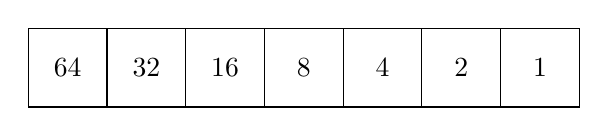
\begin{tikzpicture}
		\draw (-1,1) rectangle (0,0) rectangle (1,1) rectangle (2,0) rectangle (3,1) rectangle (4,0) rectangle (5,1) rectangle (6,0);
		\draw (5.5,0.5) node {$1$};
		\draw (4.5,0.5) node {$2$};
		\draw (3.5,0.5) node {$4$};
		\draw (2.5,0.5) node {$8$};
		\draw (1.5,0.5) node {$16$};
		\draw (0.5,0.5) node {$32$};
		\draw (-.5,0.5) node {$64$};
		
	\end{tikzpicture}
\end{center}

Ensuite, nous plaçons le nombre en binaire sous cette grille en mettant bien le chiffre des unités sous le carré le plus à droite et nous barrons les cases dont le chiffre associé est 0:

\begin{center}
	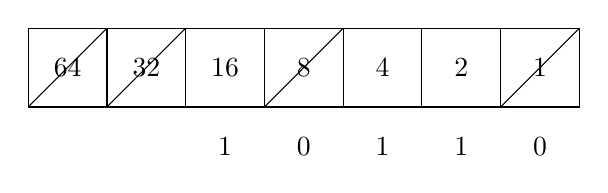
\begin{tikzpicture}
		\draw (-1,1) rectangle (0,0) rectangle (1,1) rectangle (2,0) rectangle (3,1) rectangle (4,0) rectangle (5,1) rectangle (6,0);
		\draw (5.5,0.5) node {$1$};
		\draw (4.5,0.5) node {$2$};
		\draw (3.5,0.5) node {$4$};
		\draw (2.5,0.5) node {$8$};
		\draw (1.5,0.5) node {$16$};
		\draw (0.5,0.5) node {$32$};
		\draw (-.5,0.5) node {$64$};
		
		\draw (5.5,-0.5) node {$0$};
		\draw (4.5,-0.5) node {$1$};
		\draw (3.5,-0.5) node {$1$};
		\draw (2.5,-0.5) node {$0$};
		\draw (1.5,-0.5) node {$1$};
		\draw (0.5,-0.5) node {$ $};
		\draw (-.5,-0.5) node {$ $};
		
		\draw (-1,0) -- (0,1)
		(0,0) -- (1,1)
		(2,0) -- (3,1)
		(5,0) -- (6,1);
		
	\end{tikzpicture}
\end{center}

Il ne reste plus qu'à additionner les nombres qui restent: $16 + 4 + 2=22$


\begin{myexamples}
	\item En décimal le nombre binaire $1100_{2}$ s'écrit
		  \vspace{1.5cm}
    \item En décimal le nombre binaire $10111_{2}$ s'écrit
    \vspace{1.5cm}
\end{myexamples}

\subsubsection{Conversion décimale binaire}

Pour trouver l'écriture binaire d'un nombre écrit en base 10, il existe principalement deux méthodes. 


\; 

La première méthode consiste à décomposer le nombre en somme de puissance de 2 et à utiliser la grille précédente. 

Plus concrètement, si nous voulons écrite 99 en binaire. La plus grande puissance de 2 que nous pouvons prendre dans 99 est 64 (128, la suivante, est trop grande). Il reste ensuite: 99-64=35. Dans 35 on peut mettre 32, et il restera 35-33=3. Dans 3 on ne peut ni mettre 16, ni mettre 8, ni mettre 4. On peut mettre 2. Il reste 1. Dans 1 on peut mettre 1. 

Cela signifie que 99=64+32+2+1. Sur notre grille cela donne:

\begin{center}
	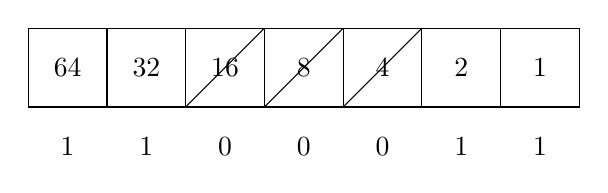
\begin{tikzpicture}
		\draw (-1,1) rectangle (0,0) rectangle (1,1) rectangle (2,0) rectangle (3,1) rectangle (4,0) rectangle (5,1) rectangle (6,0);
		\draw (5.5,0.5) node {$1$};
		\draw (4.5,0.5) node {$2$};
		\draw (3.5,0.5) node {$4$};
		\draw (2.5,0.5) node {$8$};
		\draw (1.5,0.5) node {$16$};
		\draw (0.5,0.5) node {$32$};
		\draw (-.5,0.5) node {$64$};
		
		\draw (5.5,-0.5) node {$1$};
		\draw (4.5,-0.5) node {$1$};
		\draw (3.5,-0.5) node {$0$};
		\draw (2.5,-0.5) node {$0$};
		\draw (1.5,-0.5) node {$0$};
		\draw (0.5,-0.5) node {$1$};
		\draw (-.5,-0.5) node {$1$};
		
		\draw (1,0) -- +(1,1)
		(2,0) -- +(1,1)
		(3,0) -- +(1,1)
		;
		
	\end{tikzpicture}
\end{center}

Donc $99_{(10)}=1100011_{(2)}$.


\;

La deuxième méthode consiste  effectuer des divisions successives par 2. Le nombre en binaire se lira à l'aide des restes des différentes divisions:

\begin{figure}[h]
	\begin{center}
		\includegraphics[scale=.5]{Images/intro/divisionbinaire}
	\end{center}
\end{figure}

Ainsi, $79_{(10)}=1001111_{(2)}$

\begin{myexamples}
	\item En binaire, le nombre décimal 10 s'écrit
	\vspace{3cm}
	\item En binaire, le nombre décimal 58 s'écrit
	\vspace{3cm}	
\end{myexamples}

\subsection{La base hexadécimal}
Il 
C'est le code utilisé dans la programmation de certains automates et microprocesseurs. Il est composé de : 10 chiffres de 0 à 9, et 6 lettres de A à F. Les adresse MAC (adresses unique associée à chaque carte réseau dans le monde) sont aussi écrite en base hexadécimal.

La manipulation des nombres écrits en binaire est difficile pour l'être humain et la conversion en décimal n'est pas simple. C'est pourquoi nous utilisons de préférence le système hexadécimal (base 16). 

Le tableau ci-dessous montre la représentation des nombres de 0 à 15 dans les bases 10, 2 et 16.

\begin{figure}[h]
	\begin{center}
		\includegraphics[scale=.5]{Images/intro/tableaubase}
	\end{center}
\end{figure}


Par exemple, $B4F_{(16)}= B \cdot 16^2 + 4 \cdot 16^1 + F\cdot 16^0= 11 \cdot 16^2 + 4 \cdot 16^1 + 15\cdot 16^0=2 895_{(16)}$

\subsubsection{Conversion en binaire}

Pour convertir un nombre binaire en hexadécimal il suffit de remarquer que chaque groupe de 4 bits représentes un chiffre en hexadécimal:

\begin{figure}[h]
	\begin{center}
		\includegraphics[scale=.5]{Images/intro/hexadecimal}
	\end{center}
\end{figure}

\begin{myexample}
	Le  nombre binaire $101000111100_{(2)}$ s'écrit en base hexadécimal :
	\vspace{2cm}

\end{myexample}

\subsubsection{Conversion en décimal}

La méthodes par divisions (par 16) s'applique comme en binaire (par 2).

